\documentclass[12pt]{article}
\usepackage{geometry}
\usepackage{amsmath}
\usepackage{mathtools}
\usepackage{amssymb}
\usepackage{enumitem}
\usepackage{fancyhdr}
\usepackage{tikz}
\usepackage{color}
\usepackage{xspace}
\usepackage{thumbpdf}
\usepackage{listings}
\usepackage{verbatim}
\usepackage{hyperref}
\usepackage{booktabs}
\usepackage{colortbl}
\usetikzlibrary{trees}
\usetikzlibrary{shapes,arrows}
\pagestyle{fancy}

\newcommand{\xref}[1]{\S\ref{#1}}
\definecolor{darkred}{rgb}{0.7,0,0}
\definecolor{darkgreen}{rgb}{0,0.5,0}
\hypersetup{colorlinks=true,
	linkcolor=darkred,
	citecolor=darkgreen}

\lstset{
	basicstyle=\ttfamily,
	mathescape
}

\lstdefinestyle{customc}{
	belowcaptionskip=1\baselineskip,
	breaklines=true,
	% xleftmargin=20pt,
	language=matlab,
	% frame=L,
	escapeinside={@}{@},
	showstringspaces=false,
	basicstyle=\small\ttfamily,
	keywordstyle=\bfseries\color{green!40!black},
	commentstyle=\itshape\color{purple!40!black},
	%identifierstyle=\color{blue},
	stringstyle=\color{orange},
	% directivestyle=\color{brown},
	%numbers=left,
	%numberstyle=\tiny\color{gray}
}

\lstdefinestyle{customctable}{
	aboveskip=-\medskipamount,
	belowskip=-\medskipamount,
	language=C,
	escapeinside={@}{@},
	showstringspaces=false,
	basicstyle=\scriptsize\ttfamily,
	keywordstyle=\bfseries\color{green!40!black},
	commentstyle=\itshape\color{purple!40!black},
	%identifierstyle=\color{blue},
	stringstyle=\color{orange},
	directivestyle=\color{brown},
}

\makeatletter
\renewcommand*\env@matrix[1][*\c@MaxMatrixCols c]{%
	\hskip -\arraycolsep
	\let\@ifnextchar\new@ifnextchar
	\array{#1}}
\makeatother

\newcommand*{\vertbar}{\rule[-1ex]{0.5pt}{2.5ex}}
\newcommand*{\horzbar}{\rule[.5ex]{2.5ex}{0.5pt}}

\textheight=8.5in

\newcommand{\hongzi}[1]{{{\color{red}(HM: #1)}}}

\lhead{6.854 Pset 8}
\chead{Hongzi Mao \:\: \footnotesize{collaborators:} Kevin Yang}
\rhead{Nov 2, 2016}

\begin{document}
	
\section*{Problem 1}
\paragraph{(a)} From multivariable calculus and the assumption that $A$ being symmetric, we know for $f(x) = x^T Ax - 2 b^T x$, the gradient\footnote{A quick way of deriving this is by observing $(x + \delta)^TA(x + \delta) - x^T A x= x^TA\delta + \delta^TAx + O(|\delta|^2)$. By dividing (elementwise in $\delta$) it with $\delta$ and let $\delta \to 0$, we got the derivative $(A + A^T)x$. $\nabla b^Tx = b$ is straightforward from the definition.} is 
\begin{align*}
\nabla f(x) = (A + A^T)x - 2b = 2Ax - 2b.
\end{align*}

In addition, we know when the multivariable function reaches minimum (global minimum in this context, as the function is convex), the gradient is $0$. Therefore we know at the optimum point $x*$, $\nabla f(x^*) = 0$, which leads to $2Ax^*-2b = 0$ and lets us solve $Ax = b$. 

The gradient being $0$ only makes sense when the solution is feasible. In order words, we need to show the minimum of $f(x)$ can only be finite. This can be shown by contradiction. Suppose the minimum is $-\infty$, it can only occurs when $x\to -\infty$ or $x \to \infty$, because for any finite $x$, $f(x)$ is finite. Since $A$ is positive semidefinite we know for any $x$, $x^TAx$ is non-negative.  In order words, all the eigenvalue of $A$ is non-negative. For orthogonal eigenvectors $x_1, x_2, ..., x_n$, and eigenvalues $\gamma_1, \gamma_2, ..., \gamma_n$, and $x=c_1x_1 + c_2x_2, + ... + c_nx_n$, we have $x^TAx = \gamma_1 c_1^2x_1^2 + \gamma_2 c_2^2x_2^2 + ... + \gamma_n c_n^2 x_n^2$. Since all $\gamma$'s are non-negative, this sum is overwhelmly larger than $b_1x_1 + b_2x_2 + ... + b_nx_n$, when $x \to \pm\infty$, which contradicts with the assumption that the sum of the two can go to $-\infty$.

The only exception in the last example is that some eigenvalue can be $0$ can we only extend that part of eigenvector to be $\infty$, then the sum of the matrix $A$ part will not overwhelm $bx$. Notice that in that case $Ax = \sum_{\gamma_i=0}\gamma_ix_i =0$ and $Ax=b$ would not be solvable except the trivial case $b=0$. $\square$

\paragraph{(b)}
Write out the eigenvalues of $A$ in the descending order $\gamma_1, \gamma_2, ..., \gamma_n$, and corresponding orthogonal eigenvectors $x_1, x_2, ..., x_n$. Suppose $x=c_1x_1 + c_2x_2, + ... + c_nx_n$. Then we have
\begin{align*}
\frac{||Ax||_2}{||x||_2} = \frac{||\gamma_1c_1x_1 + \gamma_2c_2x_2 + ... + \gamma_nc_nx_n||_2}{||c_1x_1 + c_2x_2 + ... + c_nx_n||_2} \leq \frac{||\gamma_1c_1x_1 + \gamma_1c_2x_2 + ... + \gamma_1c_nx_n||_2}{||c_1x_1 + c_2x_2 + ... + c_nx_n||_2} = \gamma_1. 
\end{align*}

Notice that the above inequality can saturate when we pick $x = x_1$, i.e., the eigenvector corresponding to the largest eigenvalue. Therefore, we conclude that $\Large({||Ax||_2}/{||x||_2}\Large)_{\text{max}} = \gamma_1$.

\paragraph{(c)}
Express $r^{(t)}$ in terms of $r^{(t-1)}$ as 
\begin{align*}
r^{(t)} &= A x^{(t)} - b \\
&= A\left[x^{(t-1)} - \eta\nabla f(x^{(t-1)})\right] - b \\
&= r^{(t-1)} - \eta A\left[2A^Tx^{(t-1)}-2b\right]\\
&= \large(1- 2\eta A\large) r^{(t-1)}
\end{align*}

Now use $\eta = 1/(2||A||_2)$ and take $\ell_2$ norm
\begin{align*}
||r^{(t)}||_2 &= ||\large(1- 2\eta A\large) r^{(t-1)}||_2\\
&= \|\Big|\left(1 - \frac{A}{||A||_2}\right)r^{(t-1)}\Big|\Big|_2\\
&\leq \Big|\Big|\left(1 - \frac{A}{||A||_2}\right)\Big|\Big|_2 \Big|\Big| r^{(t-1)}\Big|\Big|_2
\end{align*}

To use the condition number of $A$, we observe
\begin{align*}
\Big|\Big|\left(1 - \frac{A}{||A||_2}\right)\Big|\Big|_2 &= \text{max}_{x\neq0} \frac{\Big|\Big|\left(1 - \frac{A}{||A||_2}\right) x\Big|\Big|_2}{||x||_2}\\
& = \text{max}_{x\neq0} \frac{\Big|\Big|\left(1 - \frac{A}{||A||_2}\right) (c_1x_1 + c_2x_2 + ... + c_nx_n)\Big|\Big|_2}{||c_1x_1 + c_2x_2 + ... + c_nx_n||_2}\\
& = \text{max}_{x\neq0} \frac{\Big|\Big|c_1x_1 + c_2x_2 + ... + c_nx_n - \frac{1}{||A||_2}(\gamma_1c_1x_1 + \gamma_2c_2x_2 + ... + \gamma_nc_nx_n)\Big|\Big|_2}{||c_1x_1 + c_2x_2 + ... + c_nx_n||_2}\\
& \leq \text{max}_{x\neq0} \frac{\Big|\Big|c_1x_1 + c_2x_2 + ... + c_nx_n - \frac{1}{||A||_2}(\gamma_nc_1x_1 + \gamma_nc_2x_2 + ... + \gamma_nc_nx_n)\Big|\Big|_2}{||c_1x_1 + c_2x_2 + ... + c_nx_n||_2}\\
&= 1 - \frac{\gamma_n}{\gamma_1}\\
&= 1 - \frac{1}{\kappa(A)},
\end{align*}
where the inequality actually can stature when picking $x = x_n$. Therefore we reach the desire conclusion. $\square$

\paragraph{(d)} To show $||A\tilde{x} -b || < \epsilon$, we essentially need to find a $t$ such that $||r^{(t)}|| < \epsilon$. Notice that from $(c)$ we have 
\begin{align*}
||r^{(t)}||_2 &\leq \left(1 - \frac{1}{\kappa(A)}\right) ||r^{(t-1)}||_2 \\
&\leq \left(1 - \frac{1}{\kappa(A)}\right)^2 ||r^{(t-2)}||_2 \\
&\leq ...\\
&\leq \left(1 - \frac{1}{\kappa(A)}\right)^t ||r^{(0)}||_2 \\
\end{align*}
Now if we set $t = log_{1 - \frac{1}{\kappa(A)}}\frac{\epsilon}{||r^{(0)}||_2} = log_{\frac{\kappa(A)}{\kappa(A) - 1}}\frac{||r^{(0)}||_2}{\epsilon}$, we will have $||r^{(t)}||_2 \leq \epsilon$. Suppose other operations are in the same order of outputting the vector, $O(n)$. Therefore the running time for a good enough solution is in the order of $O(n\:log_{\frac{\kappa(A)}{\kappa(A) - 1}}(||r^{(0)}||_2/\epsilon))$. 

In fact, we can pick the initial $x^{(0)}=0$ such that $||r^{(0)}||_2 = ||b||_2$. Therefore the running time we got is $O(n\:log_{\frac{\kappa(A)}{\kappa(A) - 1}}(||r^{(0)}||_2/\epsilon))$.

\paragraph{(e)} From (d) we know for running time in the scale of $O(log(1/\epsilon))$ we can achieve $||Ax -b ||_2 < \epsilon$. From (a) we know $Ax^* = b $. Then we have 
\begin{align*}
||(Ax -b) ||_2 = ||(Ax -b) - (Ax^* -b)||_2 = |(A (x - x^*) ||_2 \leq \epsilon
\end{align*}

Since we know $A$ is invertible, we can set $\epsilon$ to be $\epsilon / ||A^{-1}||_2$, multiplying $||A^{-1}||_2$ on both end of the above inequality, we have 
\begin{align*}
||x - x^* ||_2 = ||A^{-1}A (x - x^*) ||_2 \leq ||A^{-1}||_2 ||A (x - x^*) ||_2 \leq ||A^{-1}||_2 \frac{\epsilon}{||A^{-1}||_2}
\end{align*}

Hence, we need $O(n\:log_{\frac{\kappa(A)}{\kappa(A) - 1}}(||A^{-1}||_2||r^{(0)}||_2/\epsilon))$ running time to reach $||x - x^* ||_2  \leq \epsilon$.

\paragraph{(f)} The intuition is that when $Ax$ is close to $b$, $x$ is close to a $x^*$ that solves $Ax - b$. Part (a) still works as it does not involve the assumption of $A$ being invertible. Similarly, the argument in (b) still works. For lateral parts, notice the following fact of non-invertible matrix $A$. $A$ has an invertible part $A^{+}$ and a null part $A^{0}$. $Ax = b$ only include the invertible part of $A$, i.e., $A^{+}x = b$ and $A^{0}x = 0$. Then the whole problem above can still work when we only consider the invertible part. In part (c), the new $\kappa$ only uses the minimum eigenvalue of the invertible part, which is the minimum nonzero eigenvalue of $A$. For part (d) and (e) the time bound analysis still apply following (c).\footnote{Received the hint from TA afterwards, the approach here is essentially taking the pseudoinverse $A^+$.}

\newpage
\section*{Problem 2}
\paragraph{(a)} To show the problem is of the desired form, it is sufficient to show $Ax \geq 0$ is a convex set, denoted as $S$. This can be shown by checking any $x, y \in S$. This means $Ax \geq 0$ and $Ay \geq 0$. Then for any $\lambda \in [0,1]$, $A (\lambda x + (1-\lambda)y) = \lambda Ax + (1-\lambda)Ay \geq 0.$ This is because $\lambda \geq 0$ and $(1-\lambda) \geq 0$. Therefore $(\lambda x + (1-\lambda)y) \in S$ as well. Hence $Ax\geq 0$ is a convex set. $\square$

\paragraph{(b)} Denote the contraction coefficient for $g$ and $h$ to be $w_g, w_h$, respectively. Then for any $x,y \in \mathbb{R}^n$,
\begin{align*}
||g(h(x)) - g(h(y))||_2 \leq w_g ||h(x) - h(y)||_2 \leq w_g w_h ||x - y||_2
\end{align*}
Therefore, $w_g w_h$, the product of contraction coeffiction of $g$ and $h$, is suitable for all $x, y$. The actual contraction coefficient for $g\cdot h$ would be at most $w_g w_h$. $\square$

\paragraph{(c)} Noted.
\paragraph{(d)} For $x, y$ we write out 
\begin{align*}
||g(x) - g(y)||_2 &= ||(x - \eta \nabla f(x)) - (y - \eta \nabla f(y))||_2\\
&= || (x-y) - \eta\left(\nabla f(x) - \nabla f(y)\right) ||_2\\
&= || (x-y) - \eta Z\left(x - y\right) ||_2\\
&\leq (1 - \eta \gamma_n) || x-y ||_2
\end{align*}
where $\gamma_n$ is the smallest eigenvalue\footnote{The inequality is shown in 1(c).} of $Z$. Notice that $\eta$ is selected as $1/\beta$. Recall the definition of $\beta$-smoothness $||\nabla f(x) - \nabla f(y) || \leq \beta ||x - y||$. Then we have for \emph{any} $x$ and $y$, 
\begin{align*}
||Z(x-y)||_2 = ||\nabla f(x) - \nabla f(y) ||_2 \leq \beta ||x - y||_2,
\end{align*}
in order words, $||Z(x-y)||_2/||x - y||_2 \leq \beta$. We know $\beta$ is therefore the largest eigenvalue\footnote{Proof is shown in 1(b).} of $Z$. 

Hence we reach 
\begin{align*}
||g(x) - g(y)||_2 &\leq \left(1 - \frac{\gamma_n}{\gamma_1}\right) || x-y ||_2 = \left(1 - \frac{1}{\kappa(Z)}\right) || x-y ||_2 \leq \left(1-\frac{1}{\kappa(f)}\right) || x-y ||_2
\end{align*}

Therefore, the contraction coefficient is at most $1-\frac{1}{\kappa(f)}$. $\square$

\paragraph{(e)} We prove this by contradiction. Suppose there are two different points $y, z$ in the convex set having same minimum $\ell_2$ distance to $x$. Then we know $\lambda y + (1-\lambda)z$ is also in the set $S$. Also, 

\begin{align*}
||\lambda y + (1-\lambda)z - x||_2 & = ||\lambda y - \lambda x + (1-\lambda)z - (1-\lambda)x||_2 \\
&< ||\lambda y - \lambda x ||_2 + ||(1-\lambda)z - (1-\lambda)x||_2\\
&= \lambda || y-x||_2 + (1-\lambda) ||z-x||_2\\
&= ||y-x||_2
\end{align*}

The inequality is from the triangle inequality. Notice that vector $(y-x)$ and $(z-x)$ are in different direction (if they are in the same direction, then there can only be closest point to $x$ on a single direction), the $\ell_2$ norm of the sum two different direction vector is \emph{straightly} smaller than sum of the $\ell_2$ norm of each one of them. This reaches the contradiction with the assumption that $||y-x||_2$ is minimum for all points in the convex set $S$. $\square$

\paragraph{(f)} For any $x$ and $y$, we utilize what we derived in (d) and 

\begin{align*}
\text{$\prod$}_S(x) - \text{$\prod$}_S(y) &= \text{argmin}_z ||z-x||_2 - \text{argmin}_w ||w-y||_2 \\
&\leq ||w-x||_2 - ||w-y||_2\\
&\leq ||(w-x) - (w-y)||_2\\
&= ||x-y||_2.
\end{align*}
where $w$ is taken two be the \emph{argmin} w.r.t. $y$ above. Hence $\prod_S$ is a contraction operation. $\square$

\paragraph{(g)} From part (d) we know the contraction coefficient for $g(x) = x - \eta \nabla f(x)$ is at most $1-\frac{1}{\kappa(f)}$. From part (f) we know $\prod_S$ is a contraction operation, therefore its contraction coefficient is at most $1$. From part (b) we know the composition of two contraction operation is also a contraction operation, with the contraction coefficient at most the product of each. Hence we know $\prod_S(g(x))$ is also a contraction operation, with the contraction coefficient at most $1-\frac{1}{\kappa(f)}$.

Now, consider the optimal solution $x^*$. At step $t$, the $\ell_2$ distance for $x^{(t)}$ to the optimal solution is $||x^{(t)} - x^*||_2$. Then we apply the method in part (e), then $x$ will be transformed to $x^{(t+1)}=\prod_S(g(x^{(t)}))$. If now we can show $\prod_S(g(x^*))$ is mapped to $x^*$, from the contraction operation and the corresponding coefficient above, we know at each step $x$ will be brought closer to optimal $x^*$ by a factor of $1-\frac{1}{\kappa(f)}$ or better.

To prove $\prod_S(g(x^*)) = x^*$, consider first the special case where the gradient at $x^*$ is $0$. In this case, $\prod_S(g(x^*)) = \prod_S(x^*)$. Since $x^*$ is in $S$, we know $\prod_S(x^*)$ returns $x^*$. 

Then consider the case where the gradient is nonzero. Specifically, from the hint, consider the hyperplane that contains $x^*$ and is orthogonal to the gradient at $x^*$. We need to prove that $S$ must lie entirely on one side (inclusive) of this hyperplane. This is because if $S$ does not hold above, then we can take a very small step in some direction that decreases the value of $f$, contradicting optimality. More formally,  since $f(x + \delta) - f(x) \leq [\nabla f(x)]^T \delta  +  \beta/2 ||\delta||^2$, we can choose a direction of $\delta$ in the direction that results in a \emph{negative} $[\nabla f(x)]^T \delta$ (this is feasible because part of the hyperplane containing $x$ is not orthogonal to $\nabla f(x)$). Then we make the $\delta$ small enough, such that the negative linear term predominant the quadratic term. Thus, we construct a way of decreasing the value of $f$, contradicting optimality.

\paragraph{(h)} At each time step, we do a gradient descent and then take a projection step, results in a $1-\frac{1}{\kappa(f)}$ factor improvement to the optimal $x^*$. Therefore, after $t$ steps, we will have the $\ell_2$ distance to optimal solution 

\begin{align*}
\left(1-\frac{1}{\kappa(f)}\right)^t||x_0 - x^*||_2
\end{align*}
We need to set 
\begin{align*}
t = \text{log}_{1-\frac{1}{\kappa(f)}}\frac{\epsilon}{ ||x_0 - x^*||_2}
\end{align*}
to make the $\ell_2$ distance $\epsilon$.

In each step, the projection of gradient takes at least $O(n)$ time, where $n$ is the number of entries in the vector $x$. Therefore, the running time is in the order of $O\left(n \:\text{log}_{\frac{\kappa(A)}{\kappa(A) - 1}}(||x_0 - x^*||_2/\epsilon)\right)$. 

\newpage
\section*{Problem 3}
\paragraph{(a)} Strongly convex says there exists $\alpha >0$, such that for any $x, y$, $y^T \nabla^2 f(x) y \geq \alpha ||y||^2$. In order words, the smallest eigenvalue of $\nabla^2 f(x)$ is always larger than $\alpha$. In the class, we have an equivalent condition for $\alpha$-strong convexity, An equivalent condition is $f(y)\geq f(x)+\nabla f(x)^{T}(y-x)+{\frac {\alpha}{2}}\|y-x\|_{2}^{2}$. This also graphically means strongly convex function is lower bounded by a quadratic bowl $\frac{\alpha}{2}\|y-x\|_{2}^{2}$. 

Therefore, we can construct a convex cone as $f(x) = ||x||$. It is convex because $||\lambda x + (1-\lambda) y|| < \lambda ||x|| + (1-\lambda) ||y||$ following the triangle inequality. The unique minimum is $x=0$. $f(x)$ is not strongly convex because for any $\alpha >0$, there is an $x$ such the the quadratic term overwhelms the linear term, hence $f(x)$ cannot be always above any quadratic bowl.

\begin{figure}[h!]
	\centering
	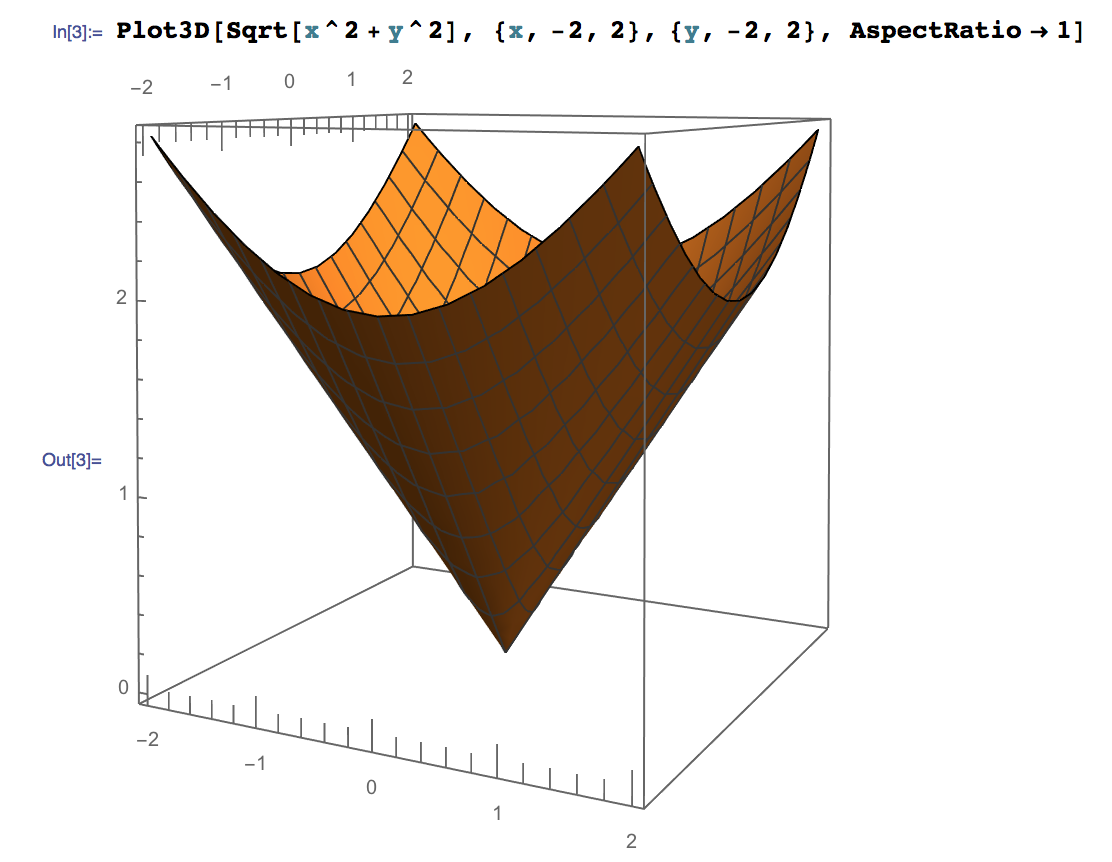
\includegraphics[width=0.7\textwidth]{3-1.png}
	\label{fig:3-1}
\end{figure}

\paragraph{(b)} For symmetric matrix $A$ and $B$, the minimum eigenvalue of the sum of them can be written as $\text{min}_{x\neq0}\frac{||(A+B)x||_2}{||x||_2} $, where the actual value can be achieved by setting $x$ to be the eigenvector corresponding to the minimum eigenvalue\footnote{Full derivation is similar to Problem 1(b). }. Also, we have
\begin{align*}
\frac{||(A+B)x||_2}{||x||_2} &= \frac{||Ax+Bx||_2}{||x||_2}\\
&=\frac{|| (c^A_1\gamma^A_1x^A_1 + c^A_2\gamma^A_2x^A_2 + ... + c^A_n\gamma^A_nx^A_n) + (c^B_1\gamma^B_1x^B_1 + c^B_2\gamma^B_2x^B_2 + ... + c^B_n\gamma^B_nx^B_n)||_2}{||x||_2} \\
&\geq \frac{|| (c^A_1\gamma^A_nx^A_1 + c^A_2\gamma^A_nx^A_2 + ... + c^A_n\gamma^A_nx^A_n) + (c^B_1\gamma^B_nx^B_1 + c^B_2\gamma^B_nx^B_2 + ... + c^B_n\gamma^B_nx^B_n)||_2}{||x||_2}\\
&=\frac{||\gamma_n^A x + \gamma_n^B x ||_2}{||x||_2}\\
&=\gamma_n^A + \gamma_n^B
\end{align*}
where $\gamma^A$'s and $\gamma_B$'s are in descending order. Therefore the minimum eigenvalue of the sum of a pair of symmetric matrices is at least the sum of their minimum eigenvalues. $\square$

\paragraph{(c)} Suppose the component for vector $x$ is $\xi_1, \xi_2, ..., \xi_n$, then $||x||^2 = (\xi_1^2 + \xi_2^2 + ... + \xi_n^2)$. Notice that $\partial ||x||^2 / \partial \xi_i\partial\xi_j = 2$ if $i = j$ and $\partial ||x||^2 / \partial \xi_i\partial\xi_j = 0$ otherwise. Hence the Hessian of $||x||^2$ is a diagonal matrix with entries on the diagonal $2$, and $0$ elsewhere. Therefore, the smallest eigenvalue of $\nabla^2 \alpha ||x||^2$ is $2\alpha$, which is the lower bound of strong convexity of $h(x)$.

\paragraph{(d)} Because $x^*$ minimizes $f(x)$, $f(x^*) \leq f(y^*)$ follows naturally. For the other part of the inequality we have $f(y^*) \leq f(y^*) + \alpha ||y^*||_2^2 \leq f(x^*) + \alpha ||x^*||_2^2$, as $y^*$ minimizes $h(x) = f(x) + \alpha ||x||^2_2$.

\paragraph{(e)} To find a $y^*$, such that $||f(y^*) - f(x^*)|| \leq \epsilon$, from (d), we know $f(x^*) \leq f(y^*) \leq f(x^*) + \alpha||x^*||^2_2$, therefore it is sufficient to reach $||f(x^*) + \alpha||x^*||^2_2- f(x^*)|| \leq \epsilon$, which is to have $\alpha||x^*||^2 \leq \epsilon$. Since we already know $||x^*|| \leq R$, we can set $\alpha = \epsilon/ R^2$. Then it suffices to look for $y^*$ that minimizes $h_{\alpha = \epsilon/ R^2}(x)$.

From part (c) we know the $h(x)$ is bounded by the smallest eigenvalue of the Hessian, which is $2\alpha = 2\epsilon / R^2$. The largest eigenvalue for $f(x)$ is $\beta + 2\alpha$.

From problem 2, we can start $x_0 = 0$ and $||x_0 - x^*|| = ||x^*|| \leq R$, the running time is bounded by $O\left(n \:\text{log}_{\frac{\kappa}{\kappa - 1}}(R/\epsilon)\right)$, where $\kappa = (\beta + 2\alpha) / 2\alpha$ and $2\alpha = 2\epsilon / R^2$. 

\newpage
\section*{Problem 4}
\paragraph{(a)} Since the optimal distance $d$ is known in a priori, we can build clusters iteratively. In each iteration, pick any point that has not been assigned to a cluster yet, and pick any free-to-assign point within $d$ distance to that point, and form a new cluster. The iterations terminate when no points all assigned to some cluster. 

From triangle inequality, since we know the points in a cluster are all within distance $d$ to the center (the one we pick first in each iteration), each point is at most within $2d$ distance to any other point in the cluster. This forms a $2$-approximation.

The iterating algorithm has to terminate before or on the $k$-th iteration. This is because we know there are $k$ clusters, each point that is not assigned to the current new cluster must has been assigned to some other cluster (within distance $d$ to that center). After $k$ iterations, the points to all $k$ clusters (in optimal case) must be assigned to some (actual) clusters. Therefore the algorithm terminates in $k$ iterations. 

\paragraph{(b)} In each iteration, the point chosen is the \emph{maximum} distance to the centers being chosen already. In the optimal clusters, any point in larger distance than $d$ is in a different cluster. Therefore in the algorithm the point being selected must be from another cluster (if it exists, its distance is the largest to all centers). Since we know there are k clusters in the optimal clustering, after k iterations, the maximum distance of points to all centers will be less than $d$. The $2$-approximation follows by the similar triangular inequality argument, where all points in a cluster have distance at most $2d$. 
\end{document}